\documentclass{book}
\usepackage[utf8]{inputenc}
\usepackage{cancel}
\usepackage[margin=2cm,a4paper]{geometry}
\usepackage{amsmath}
\usepackage{amssymb}
\usepackage{undertilde}
\usepackage{graphicx}
\usepackage{hyperref}
\usepackage{gensymb}
\usepackage{tipa}
\usepackage{pgfplots}
\usepackage[british]{babel}
\usepackage{pdfpages}
\usepackage{parskip}

\newenvironment{generalInformation}{}{}
\newenvironment{explanationOfTerms}{}{}
\newenvironment{example}{}{}
\newenvironment{note}{\begin{center}\em NOTE: \\}{\end{center}}

% user defined commands
\newcommand{\Comb}[2]{{}^{#1}C_{#2}}
\newcommand{\Perm}[2]{{}^#1P_{#2}}
\newcommand{\note}[1]{\begin{center}\emph{NOTE: {#1}}\end{center}}
\newcommand{\arc}[1]{{\setbox9=\hbox{#1}\ooalign{\resizebox{\wd9}{\height}{\texttoptiebar{\phantom{A}}}\cr#1}}}

\graphicspath{ {./images/} }

% Title Page
\title{Mathematical Specialists}
\author{Lachlan Takumi Ikeguchi}

\begin{document}
\maketitle
\tableofcontents

\section{The purpose}
This document was written to be used as a summary to help revise the content covered mathematical specialists.  For any inquiries, feedback, and further explanations, contact lachlanprivate@duck.com or through the discord server: \url{https://discord.gg/6P8rddkXFr}.  I encourage you to let me know of any topic I missed, how I could explain it better, or how it could be reworded or formatted to be more helpful in its purpose.  The goal of this document is to be a comprehensive summary of everything you need to know.

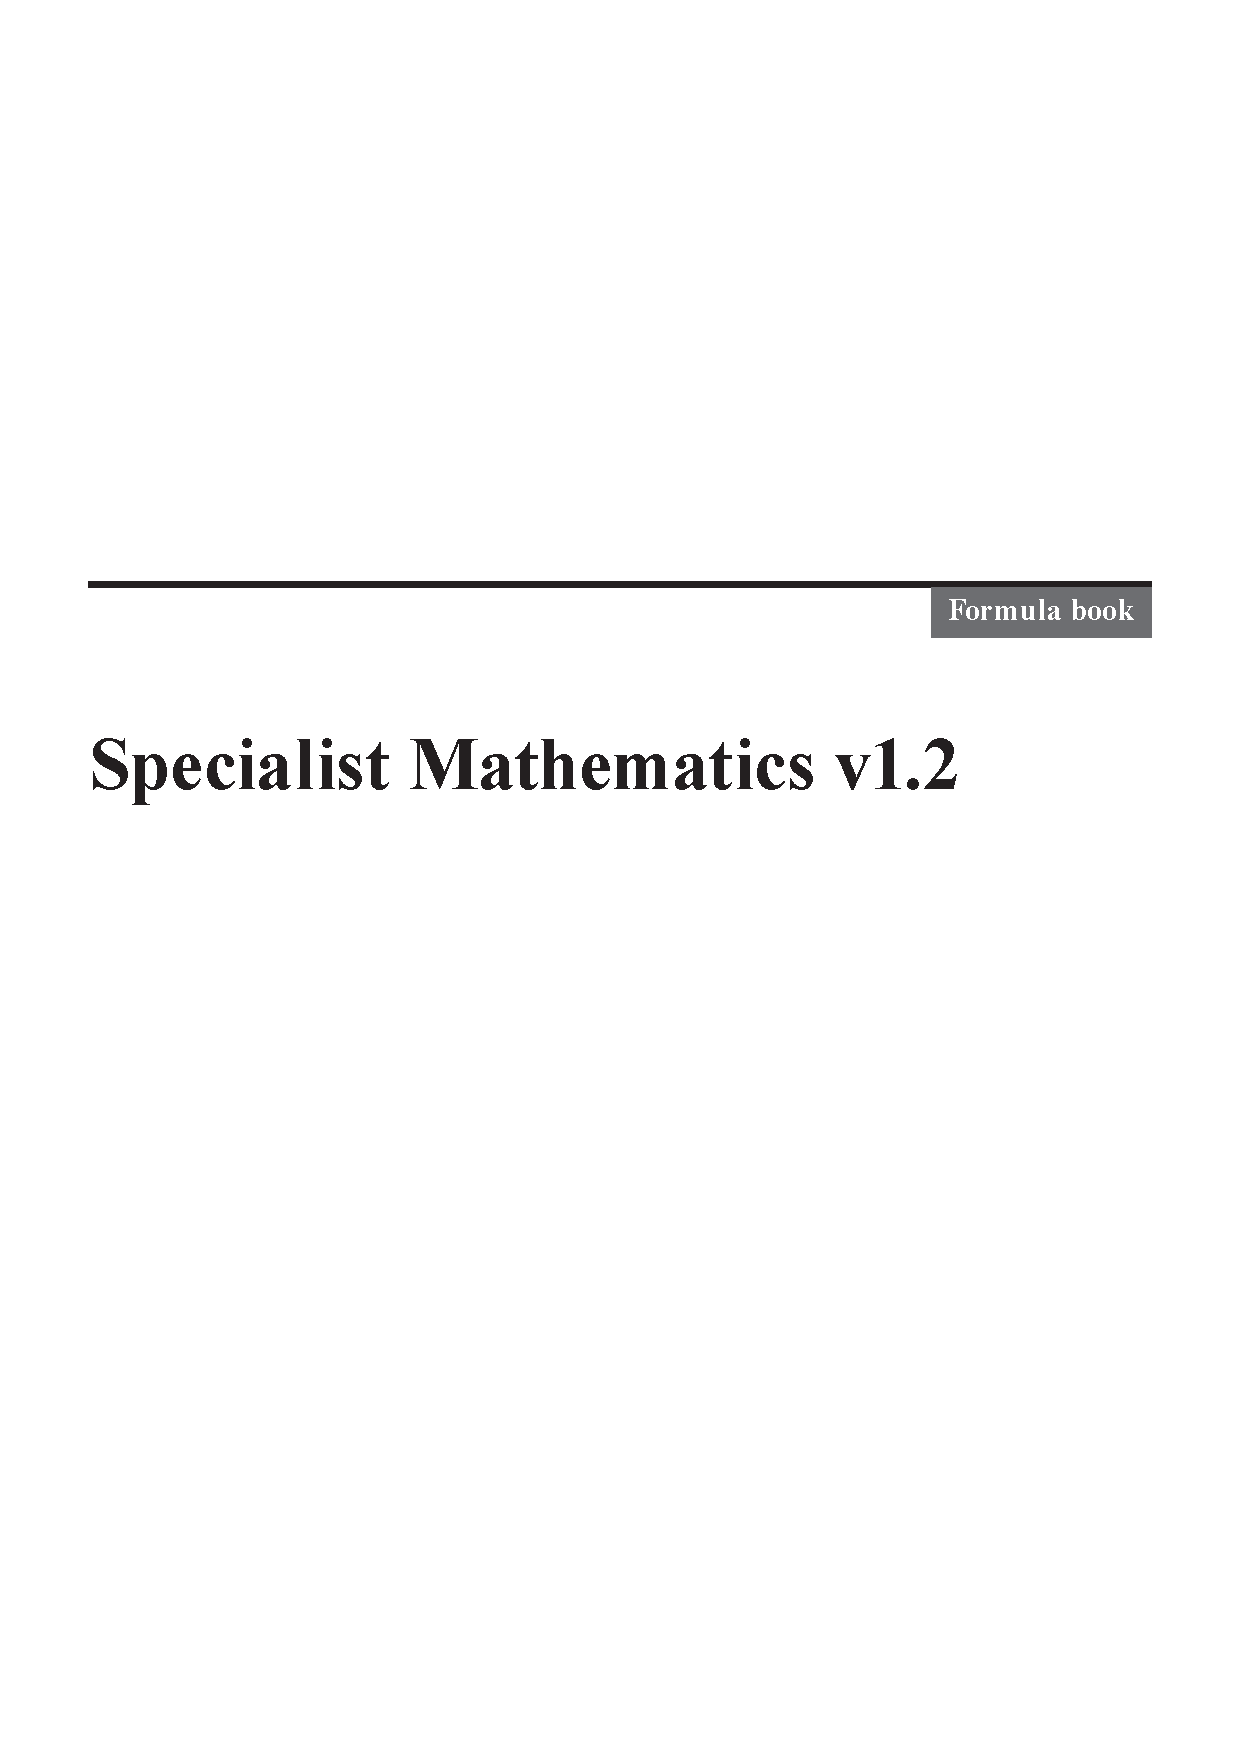
\includepdf{./images/formula-book.pdf}

\chapter{Combinatorics}
\section{Addition principle}
If there are $n$ ways of performing operation $A$, and $m$ ways of performing operation $B$, there are $n + m$ ways of performing operation $A \cap B$.

As in, let there be 2 ways to perform task $A$, and 3 ways to perform task $B$.  If there is an option to perform $A$ \emph{or} $B$, there is a total of $2 + 3 = 5$ ways to perform an operation.

\section{Multiplication principle}
If there are $n$ ways of performing operation $A$, and $m$ ways of performing operation $B$, there are $n \times m$ ways of performing operation $A \cup B$.\\

As in, let there be 4 ways to perform task $A$, and 5 ways to perform task $B$.  With considering 1 way to perform $A$, there are 5 ways to perform $B$, repeat the process through the number of ways to perform $A$.

\begin{center}
	\begin{tabular}{l|lllll}
		       & $B$, 1 & $B$, 2 & $B$, 3 & $B$, 4 & $B$, 5 \\ \hline
		$A$, 1 & (1, 1) & (1, 2) & (1, 3) & (1, 4) & (1, 5) \\
		$A$, 2 & (2, 1) & (2, 2) & (2, 3) & (2, 4) & (2, 5) \\
		$A$, 3 & (3, 1) & (3, 2) & (3, 3) & (3, 4) & (3, 5) \\
		$A$, 4 & (4, 1) & (4, 2) & (4, 3) & (4, 4) & (4, 5) \\
	\end{tabular}
\end{center}
Where there are $4 \times 5 = 20$ ways to perform the operations.

\chapter{Factorials}
Factorials is the result of multiplying all the integers between the given integer and 1.  This is given the notation and formula:
\[
	n! = n \times (n-1) \times (n-2) \times (n-3)... \times 3 \times 2 \times 1
\]
\begin{align*}
	5! & = 5 \times 4 \times 3 \times 2 \times 1 \\
	   & = 120
\end{align*}

\section{Dividing factorials}
When given some factorial over another factorial in such cases as:
\[
	\frac{4!}{2!}
\]
\[
	\frac{4 \times 3 \times 2 \times 1}{2 \times 1}
\]
\[
	\frac{4 \times 3 \times \cancel{2 \times 1}}{\cancel{2 \times 1}}
\]
\[
	4 \times 3
\]
\[
	12
\]

\section{Special cases}
\[
	0! = 1
\]

\chapter{Permutations}
Permutations is the number of ways of choosing $r$ things from $n$ distinct things where \emph{order matters}.  This is given the notation and formula:
\[
	^nP_r = \frac{n!}{(n-r)!}
\]
\begin{align*}
	\Perm{6}{4} & = \frac{6!}{(6 - 4)!}                                                                 \\
	            & = \frac{6!}{2!}                                                                       \\
	            & = \frac{6 \times 5 \times 4 \times 3 \times 2 \times 1}{2 \times 1}                   \\
	            & = \frac{6 \times 5 \times 4 \times 3 \times \cancel{2 \times 1}}{\cancel{2 \times 1}} \\
	            & = 6 \times 5 \times 4 \times 3                                                        \\
	            & = 360
\end{align*}

\section{Permutations in a circle}
In cases where the positions being concerned is a circle such as the permutations of a circular seating arrangement, if the standard permutations formula is applied, there are several over-counting of the like arrangement in a different perspective.  In these cases apply the formula:
\[
	\frac{^nP_r}{r} = \frac{\frac{n!}{(n-r)!}}{r}
\]

\section{Like objects repetitions}
The number of ways of arranging $n$ objects made up of indistinguishable objects, $n_1$ in the first group, $n_2$ in the second group and so on, is:
\[
	\frac{n!}{n_1! n_2! n_3!... n_r!}
\]

Find the number of permutations of the letters in the world WOOLLOOMOOLOO.\\
There are 8 'O's and 3 'L's\\
Permutations:
\[\frac{13!}{8!3!}\]
\[\frac{13 \times 12 \times 11 \times 10 \times 9 \times 8 \times 7 \times 6 \times 5 \times 4 \times 3 \times 2 \times 1}{(8 \times 7 \times 6 \times 5 \times 4 \times 3 \times 2 \times 1) \times (3 \times 2 \times 1)}\]
\[\frac{13 \times 12 \times 11 \times 10 \times 9 \cancel{\times 8 \times 7 \times 6 \times 5 \times 4 \times 3 \times 2 \times 1}}{\cancel{(8 \times 7 \times 6 \times 5 \times 4 \times 3 \times 2 \times 1)} \times (3 \times 2 \times 1)}\]
\[\frac{13 \times 12 \times 11 \times 10 \times 9}{3 \times 2}\]
\[\frac{13 \times \cancelto{6 \cancel{\times 2}}{12} \times 11 \times 10 \times \cancelto{3 \cancel{\times 3}}{9}}{\cancel{3 \times 2}}\]
\[13 \times 6 \times 11 \times 10 \times 3\]
\[25,740\]

\section{Restrictions}
When considering restrictions, deal with the restrictions first.\\

Find the number of arrangements of the letters of the word DARWIN beginning and ending with a vowel.\\
Number of letters = 6\\
Number of positions = 6\\
Beginning and end must be a vowel, so the available positions are decreased by 2: number of positions - 2 = 4\\
Since 2 vowels must be used:  number of letters - 2 = 4\\
Permutations:
\[\Perm{4}{4}\]
\[4!\]
\[4 \times 3 \times 2 \times 1\]
\[24\]

\section{Grouped items}
When items are grouped together, treat each group as a single object.  Find the number of arrangements of the groups, then multiply by the number of arrangement within each group.\\

Find the number of arrangement of the letters of the word EQUALS if the vowels are kept together.\\
Number of vowels = 3\\
Number of letters = 6\\
Number of positions = 6\\
As the 3 vowels are grouped together, the number of positions decreases:\\ number of positions - 3\textsubscript{for the members of the group} + 1\textsubscript{for the group} = 4\\
Permutations within vowel group:
\[^3P_3 = 3! = 3 \times 2 = 6\]
Permutations of all positions:
\[^4P_4 = 4! = 4 \times 3 \times 2 = 24\]
Multiply together:
\[6 \times 24 = 144\]

\section{Special cases}
\[^nP_n = n!\]
\[^nP_0 = 1\]

\chapter{Combinations}
Combinations is the number of ways of choosing or selecting $r$ objects from $n$ distinct objects where \emph{order does not matter}.  This is given the notation and formula:
\[^nC_r = \frac{^nP_r}{r!}\]
\[^nC_r = \frac{\frac{n!}{(n-r)!}}{r!}\]

\begin{align*}
	^4C_2 & = \frac{^4P_2}{2!}                                          \\
	      & = \frac{\frac{4!}{(4 - 2)!}}{2!}                            \\
	      & = \frac{\frac{4!}{2!}}{2!}                                  \\
	      & = \frac{\frac{4 \times 3 \times 2}{2}}{2}                   \\
	      & = \frac{\frac{4 \times 3 \cancel{\times 2}}{\cancel{2}}}{2} \\
	      & = \frac{4 \times 3}{2}                                      \\
	      & = \frac{12}{2}                                              \\
	      & = 6                                                         \\
\end{align*}

\section{Combinations with restrictions}
\subsection{Combinations with specific terms}
When given a restriction that something must be something, consider the restriction first:\\

Grace belongs to a group of 8 workers.  How many ways can a team of four workers be selected if Grace must be on the team?\\
If there is no restriction, it would be equal to $\Comb{8}{4}$.  But as Grace must be on the team, $n$ must be equal to $8 - 1$ and $r$ must be also $4 - 1$\\
Therefore, the answer is:
\[
	\Comb{7}{3} = 35
\]
35 total combinations.

\subsection{Combinations from multiple groups}
When given two combinations, multiply them together:\\

From 7 women and 4 men in a workplace, how many gropes of 5 can be chosen containing 3 women and 2 men?
Women:
\[
	\Comb{7}{3} = 35
\]
Men:
\[
	\Comb{4}{2} = 6
\]
Total:
\[
	35 \times 6 = 210
\]

\subsection{Permutations and Combinations combined}
When given two combinations, in which the output is a permutations:

How many arrangement of the letters in the word ``DUPLICATE'' can be made that have two vowels and three consonants?\\

First of all, there are 4 vowels, and 5 consonants.  And 2 vowels are selected, while 3 vowels are selected:
\[
	\Comb{4}{2} = 6
\]
\[
	\Comb{5}{3} = 10
\]
And there are $5!$ ways to arrange 5 objects, therefore
\[
	6 \times 10 \times 5! = 7200
\]

\section{Pascal's triangle}
The Pascal's triangle is a pattern formed by adding the top 2 adjacent numbers and a 1 is placed on either side of the bottom row to resemble a triangle:
\begin{center}
	\begin{tabular}{rccccccccccccccccccccc}
		$n=0$:  &   &   &    &   &    &    &     &    &     &     & 1                                                     \\\noalign{\smallskip\smallskip}
		$n=1$:  &   &   &    &   &    &    &     &    &     & 1   &     & 1                                               \\\noalign{\smallskip\smallskip}
		$n=2$:  &   &   &    &   &    &    &     &    & 1   &     & 2   &     & 1                                         \\\noalign{\smallskip\smallskip}
		$n=3$:  &   &   &    &   &    &    &     & 1  &     & 3   &     & 3   &     & 1                                   \\\noalign{\smallskip\smallskip}
		$n=4$:  &   &   &    &   &    &    & 1   &    & 4   &     & 6   &     & 4   &    & 1                              \\\noalign{\smallskip\smallskip}
		$n=5$:  &   &   &    &   &    & 1  &     & 5  &     & 10  &     & 10  &     & 5  &     & 1                        \\\noalign{\smallskip\smallskip}
		$n=6$:  &   &   &    &   & 1  &    & 6   &    & 15  &     & 20  &     & 15  &    & 6   &    & 1                   \\\noalign{\smallskip\smallskip}
		$n=7$:  &   &   &    & 1 &    & 7  &     & 21 &     & 35  &     & 35  &     & 21 &     & 7  &    & 1              \\\noalign{\smallskip\smallskip}
		$n=8$:  &   &   & 1  &   & 8  &    & 28  &    & 56  &     & 70  &     & 56  &    & 28  &    & 8  &   & 1          \\\noalign{\smallskip\smallskip}
		$n=9$:  &   & 1 &    & 9 &    & 36 &     & 84 &     & 126 &     & 126 &     & 84 &     & 36 &    & 9 &    & 1     \\\noalign{\smallskip\smallskip}
		$n=10$: & 1 &   & 10 &   & 45 &    & 120 &    & 210 &     & 252 &     & 210 &    & 120 &    & 45 &   & 10 &   & 1 \\\noalign{\smallskip\smallskip}
	\end{tabular}
\end{center}

Each element in the Pascal's triangle can be used to calculate combinations, hence, the triangle can be written using Combinations notation ($^nC_r$):
\begin{center}
	\begin{tabular}{rcccccccccccccccc}
		$n=0$: &  &  &  &  &  &         &         &         &         &         & $^0C_0$                                                   \\ \noalign{\smallskip\smallskip}
		$n=1$: &  &  &  &  &  &         &         &         &         & $^1C_0$ &         & $^1C_1$                                         \\ \noalign{\smallskip\smallskip}
		$n=2$: &  &  &  &  &  &         &         &         & $^2C_0$ &         & $^2C_1$ &         & $^2C_2$                               \\ \noalign{\smallskip\smallskip}
		$n=3$: &  &  &  &  &  &         &         & $^3C_0$ &         & $^3C_1$ &         & $^3C_2$ &         & $^3C_3$                     \\ \noalign{\smallskip\smallskip}
		$n=4$: &  &  &  &  &  &         & $^4C_0$ &         & $^4C_1$ &         & $^4C_2$ &         & $^4C_3$ &         & $^4C_4$           \\ \noalign{\smallskip\smallskip}
		$n=5$: &  &  &  &  &  & $^5C_0$ &         & $^5C_1$ &         & $^5C_2$ &         & $^5C_3$ &         & $^5C_4$ &         & $^5C_5$ \\ \noalign{\smallskip\smallskip}
	\end{tabular}
\end{center}

Pascal's triangle shows that the $r^\text{th}$ element of the $n^\text{th}$ row of Pascal's triangle is given by $^nC_r$.  It is assumed that the 1 at the beginning of each row is the $0^\text{th}$ element.  This gives the \emph{Pascal's identity}:
\[
	^nC_r = ^{n-1}C_{r-1} + ^{n-1}C_r \text{ for } 0 < r < n
\]

The Pascal's triangle can be extended to the binomial theorem, where the rule for expanding an expression such as $(a + b)^n$.  Where:
\begin{align*}
	(a + b)^0 & = 1a^0b^0                                                     \\
	(a + b)^1 & = 1a^1b^0 + 1a^0b^1                                           \\
	(a + b)^2 & = 1a^2b^0 + 2a^1b^1 + 1a^0b^2                                 \\
	(a + b)^3 & = 1a^3b^0 + 3a^2b^1 + 3a^1b^2 + 1a^0b^3                       \\
	(a + b)^4 & = 1a^4b^0 + 4a^3b^1 + 6a^2b^2 + 4a^1b^3 + 1a^0b^4             \\
	(a + b)^5 & = 1a^5b^0 + 5a^4b^1 + 10a^3b^2 + 10a^2b^3 + 5a^1b^4 + 1a^0b^5
\end{align*}

\chapter{Non-right-angle-triangles}
\section{Sine rule}
The sine rule is:
\[
	\frac{a}{\sin(A)} = \frac{b}{\sin(B)} = \frac{c}{\sin(C)}
\]
Where $a$, $b$, and $c$ are lengths of sides of a triangle, and $A$, $B$, and $C$ are angles opposite the sides.

\section{Cosine rule}
The cosine rule is:
\[
	c^2 = a^2 + b^2 -2ab\cos\theta
\]
Where $c$ is the length of side opposite $\theta$, and $a$ and $b$ are the other two sides.

\chapter{Vectors}
Vectors have a magnitude and a direction.  There are three ways for writing vectors, either the Cartesian form/component from or the polar form.  Vectors are represented by $\utilde{a}$.  the Cartesian form is written as:
\[
	\utilde{v} = \begin{bmatrix}
		0 \\
		2
	\end{bmatrix}
\]
The component form notation is written as:
\[
	\utilde{v} = 2\hat{i} + 3\hat{j}
\]
And polar from is written as:
\[
	\utilde{v} = (r, \theta)
\]
Where $r$ is the radius and $\theta$ is the direction in angles.\\

$\hat{i}$ is the unit vector in the x-axis, and $\hat{j}$ is the unit vector in the y-axis.  Unit vectors are the basis vectors and are multiplied by scalars to move the tip of the vector and represent different vectors.

\section{Addition of vectors}
Let $\utilde{a} = 3\hat{i} + -2\hat{j}$ , and $\utilde{b} = 7\hat{i} + 1\hat{j}$\\
And the addition of these vectors $\utilde{a} + \utilde{b} = \utilde{c}$\\
\begin{align*}
	\utilde{c} & = \utilde{a} + \utilde{b}                    \\
	\utilde{c} & = 3\hat{i} + -2\hat{j} + 7\hat{i} + 1\hat{j} \\
	\utilde{c} & = 10\hat{i} + -1\hat{j}
\end{align*}

\section{Multiplication of vectors by a scalar}
Let $\utilde{x} = 4\hat{i} + -5\hat{j}$\\
And $\utilde{s} = 2\utilde{x}$
\begin{align*}
	\utilde{s} & = 2\utilde{x}             \\
	\utilde{s} & = 2(4\hat{i} + -5\hat{j}) \\
	\utilde{s} & = 8\hat{i} + -10\hat{j}
\end{align*}

\section{Calculating the magnitude of a vector}
The magnitude of a vector is written as $|\utilde{v}|$, and to calculate the magnitude of a vector use the pythagoras's theorem:\\

Let $\utilde{w} = 3\hat{i} + 4\hat{j}$
\begin{align*}
	\utilde{w}   & = 3\hat{i} + 4\hat{j}  \\
	|\utilde{w}| & = \sqrt{{3}^2 + {4}^2} \\
	|\utilde{w}| & = 5
\end{align*}


\section{Calculating the angle of a vector}
To calculate the angle of a vector, use the sine, cosine, and tangent ratios.\\

The trigonometric ratio are as follows:
\begin{center}
	\begin{tabular}{c|c}
		Name    & Ratio                                       \\ \hline
		Sine    & $\frac{\text{Opposite}}{\text{Hypotenous}}$ \\
		Cosine  & $\frac{\text{Adjecent}}{\text{Hypotenous}}$ \\
		Tangent & $\frac{\text{Opposite}}{\text{Adjecent}}$
	\end{tabular}
\end{center}


Let $\utilde{a} = 3\hat{i} + 4\hat{j}$\\
To calculate the angle of $\utilde{a}$, I will use the tangent rule:
\begin{align*}
	\utilde{a}             & = 3\hat{i} + 4\hat{j} \\
	\tan\theta             & = \frac{4}{3}         \\
	\tan^{-1}(\frac{4}{3}) & = \theta              \\
	                       & = 53.1301024\degree
\end{align*}


\section{The negative of a vector}
The negative of a vector is the the vector of same length, but pointing in the opposite direction.

Let $\utilde{a} = -1\hat{i} + 3\hat{j}$\\
The inverse or the negative vector would be $-\utilde{a} = 1\hat{i} + -3\hat{j}$\\
As you can see, $\utilde{a}$ points off to the left and up, and $-\utilde{a}$ points to the right and down.


\section{Converting between component form and polar form}
To convert between the component form and polar from, use the trigonometric ratios.\\
If given a polar vector, the component form is $\utilde{v} = r\cos(\theta)\hat{i} + r\sin(\theta)\hat{j}$

\section{How to find the vector between points that is at the tip of other vectors}
If given vectors $\utilde{a}$ and $\utilde{b}$ and points $A$ and $B$ that lie at the tips of the vectors, and told to find the vector $\Vec{AB}$, it will be equal to $-\utilde{a} + \utilde{b}$.\\

Let vectors $\utilde{a} = 1\hat{i} + 4\hat{j}$, $\utilde{b} = -2\hat{i} + 0\hat{j}$, and points $A = (1, 4)$, $B = (-2, 0)$\\
To find vector $\Vec{AB}$:\\
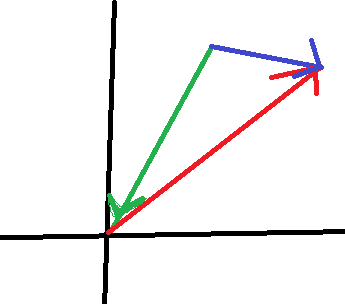
\includegraphics[scale=0.5]{VecAB}\\
Where the blue vector is $\Vec{AB}$, red is $\utilde{b}$, and green is $-\utilde{a}$


\section{Unit vectors}
To use a vector as the unit vector for others, use the formula:
\[
	\utilde{\hat{u}} = \frac{\utilde{u}}{|\utilde{u}|}
\]

\section{Dot products}
The dot product represents one vector being projected onto the other vector, and multiplying the length of the projection by the length of the other vector.  This is calculated by:
\[\utilde{a} \cdot \utilde{b} = |\utilde{a}||\utilde{b}|\cos\theta\]
or
\[\utilde{a} \cdot \utilde{b} = \utilde{a}_{\hat{i}} \utilde{b}_{\hat{i}} + \utilde{a}_{\hat{j}} \utilde{b}_{\hat{j}}\]

\note{If the result is positive, the angle between the two vectors is between 0 to 90 \degree, if it is 0, it is at 90 \degree, and if it is a negative, it is between 90 to 180 \degree.}


\section{Angle between two vectors}
Using the two formulas for calculating the dot product, the equation for cosine can be derived:
\[
	\cos\theta = \frac{\utilde{a}_{\hat{i}} \utilde{b}_{\hat{i}} + \utilde{a}_{\hat{j}} \utilde{b}_{\hat{j}}}{|\utilde{a}||\utilde{b}|}
\]

\section{Scalar resolutes}
The scalar resolute is the length of the resultant vector if it were to be projected onto the other vector where a line from the tip of the vector projected to the tip of the projection is perpendicular to the vector being projected onto:
\begin{center}
	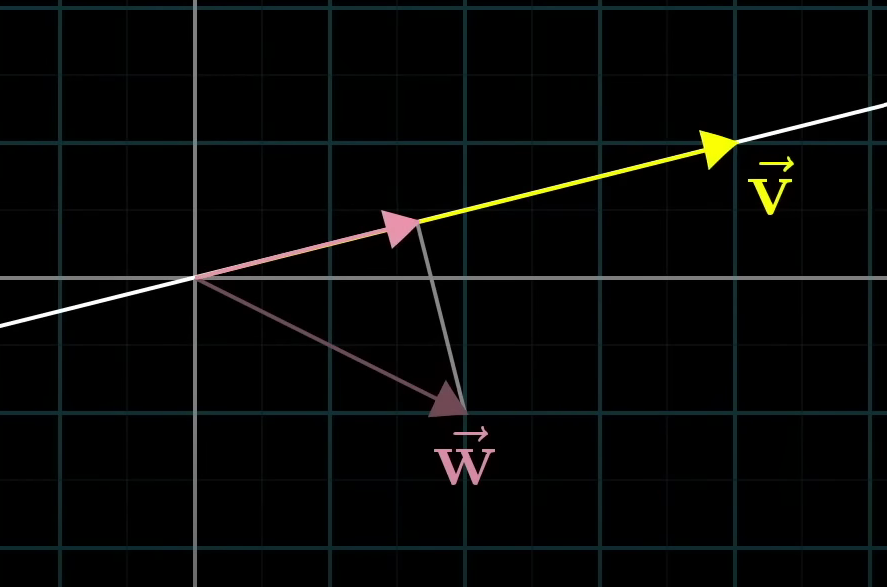
\includegraphics[scale=0.5]{dot product explination}
	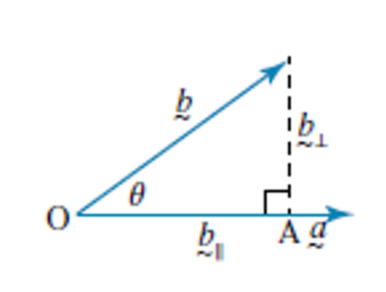
\includegraphics[scale=0.5]{dot product explination 2}
\end{center}
This can be calculated using the formula:
\[
	\Vec{OA} = |\utilde{b}|\cos\theta
\]
Where $\Vec{OA}$ is the line between the origin and the tip of the projected vector, $\utilde{b}$ is the vector being projected, and $\theta$ is the angle between the two vectors.  Or:
\[
	\Vec{OA} = \frac{\utilde{a} \cdot \utilde{b}}{|\utilde{a}|}
\]
And also:
\[
	\Vec{OA} = \hat{\utilde{a}} \cdot \utilde{b}
\]

\section{Vector resolutes}
The vector resolute is the same concept as the scalar resolute, but only that that we are concerned with the vector instead of the magnitude of the vector.  As we are projecting a vector onto another vector, we can simply multiply the result of the scalar resolute with the unit vector of the vector we are projecting onto:
\[
	\utilde{b}_{\parallel} = (\hat{\utilde{a}} \cdot \utilde{b}) \hat{\utilde{a}}
\]

Additionally, the vector perpendicular to the vector being projected to is given by:
\[
	\utilde{b}_{\perp} = \utilde{b} - (\hat{\utilde{a}} \cdot \utilde{b}) \hat{\utilde{a}}
\]

\section{Applications of vectors}
\subsection{Forces}
Use the non-right-angle-triangles rules for the triangles of forces.  And the resultant force (the vector of the actual force experienced) is the the sum of all forces (vectors) using vector addition.

\subsection{Relative vectors}
The general relationship between relative velocities is:
\[
	\utilde{v}_a = \utilde{v}_{(\text{$a$ relative to $b$})} + \utilde{v}_b
\]
Where $\utilde{v}_a$ is the actual vector and $\utilde{v}_{(\text{$a$ relative to $b$})}$ is the vector relative to $b$.

\chapter{Euclidean geometry}
There are some basic statements that are accepted as true without proving them.  In general, when these statements refer to working with numbers, the statements are called axioms.  When the statements are about geometry, they are called postulates.

\section{Postulates}
\begin{itemize}
	\item A straight line can be drawn from one point to another (that is, any two points will form a straight line)
	\item It is possible to produce a finite straight line
	\item a circle can be described with any centre and radius
	\item All right angles are equal to eachother
	\item If there is a line and a point on the line, then one line can be drawn through the point that is parallel to the original line (does not work in non-euclidean geometry)
\end{itemize}

\section{Theorems}
\begin{center}
	\begin{tabular}{|p{5cm}|p{6cm}|p{2cm}|}
		\hline
		Theorem                                                            & Diagram                                         & Symbol                                                 \\ \hline
		Adjacent angles on a straight line are supplementary.              & 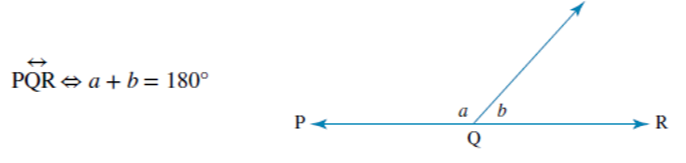
\includegraphics[width=6cm]{geometry theorem 1} & 
\includegraphics[width=2cm]{geometry theorem 1 symbol} \\ \hline
		If two lines are parallel, the corresponding angles are congruent. & 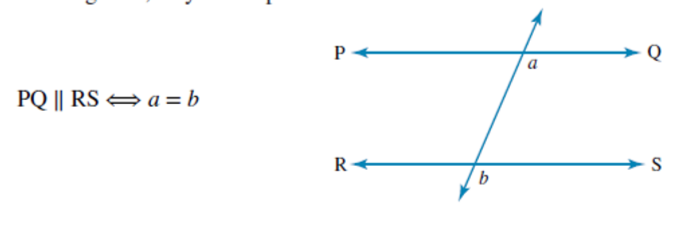
\includegraphics[width=6cm]{geometry theorem 2} & 
\includegraphics[width=2cm]{geometry theorem 2 symbol} \\ \hline
		Vertically opposite angles are congruent.                          & 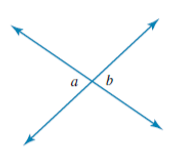
\includegraphics[width=6cm]{geometry theorem 3} & 
\includegraphics[width=2cm]{geometry theorem 3 symbol} \\ \hline
	\end{tabular}
	\begin{tabular}{|p{5cm}|p{6cm}|p{2cm}|}
		\hline
		Theorem                                                                                   & Diagram                                         & Symbol                                                 \\ \hline
		If two lines are parallel, the alternate angles are congruent.                            & 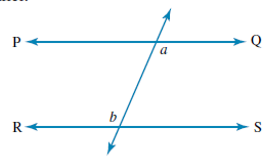
\includegraphics[width=6cm]{geometry theorem 4} & 
\includegraphics[width=2cm]{geometry theorem 4 symbol} \\ \hline
		The exterior angle of a triangle is equal to the sum of the two interior opposite angles. & 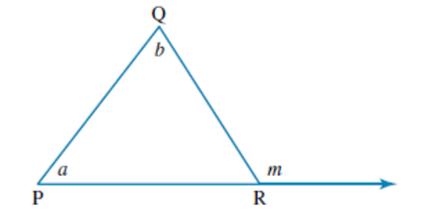
\includegraphics[width=6cm]{geometry theorem 5} & 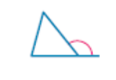
\includegraphics[width=2cm]{geometry theorem 5 symbol} \\ \hline
		The sum of the angles of a triangle is 180 \degree.                                       & 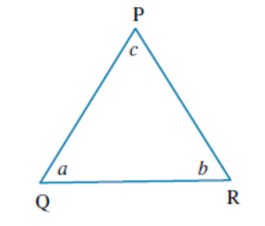
\includegraphics[width=6cm]{geometry theorem 6} & 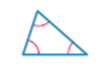
\includegraphics[width=2cm]{geometry theorem 6 symbol} \\ \hline
		In an isosceles triangle, the opposite angles are congruent.                              & 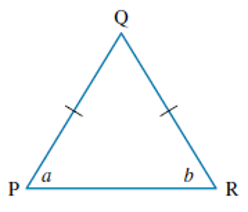
\includegraphics[width=6cm]{geometry theorem 7} & 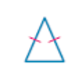
\includegraphics[width=2cm]{geometry theorem 7 symbol} \\ \hline
	\end{tabular}
	\begin{tabular}{|p{5cm}|p{6cm}|p{2cm}|}
		\hline
		Theorem                                                         & Diagram                                          & Symbol                                                  \\ \hline
		In in equilateral triangle, all sides and angles are congruent. & 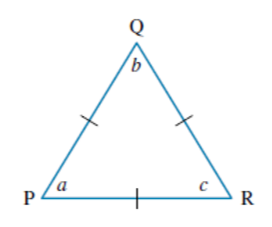
\includegraphics[width=6cm]{geometry theorem 8}  & 
\includegraphics[width=2cm]{geometry theorem 8 symbol}  \\ \hline
		The sum of the angles of a quadrilateral is 360 \degree.        & 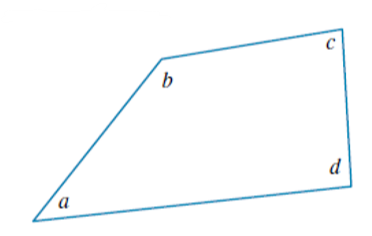
\includegraphics[width=6cm]{geometry theorem 9}  & 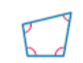
\includegraphics[width=2cm]{geometry theorem 9 symbol}  \\ \hline
		The opposite angles of a parallelogram are congruent.           & 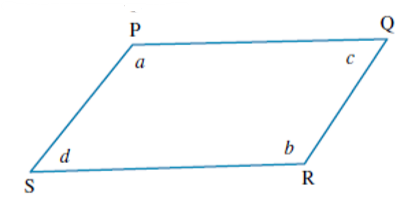
\includegraphics[width=6cm]{geometry theorem 10} & 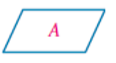
\includegraphics[width=2cm]{geometry theorem 10 symbol} \\ \hline
		Angles at a point add to 360 \degree.                           & 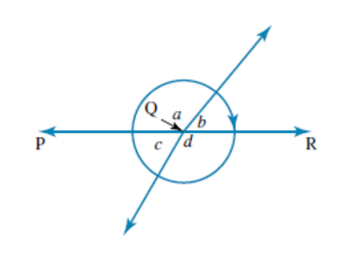
\includegraphics[width=6cm]{geometry theorem 11} & 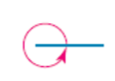
\includegraphics[width=2cm]{geometry theorem 11 symbol} \\ \hline
	\end{tabular}
\end{center}

\chapter{Proofs}
\section{Number systems}
The notation for referring to different sets of numbers are:
\begin{center}
	\begin{tabular}{c|c}
		Symbol           & Meaning           \\ \hline
		$\mathbb{R}$     & Real numbers      \\
		$\mathbb{N}$     & Natural numbers   \\
		$\mathbb{Z}$     & Integers          \\
		$\mathbb{Z}^{+}$ & Positive integers \\
		$\mathbb{Z}^{-}$ & Negative integers \\
		$\mathbb{Q}$     & Rational numbers
	\end{tabular}\\
	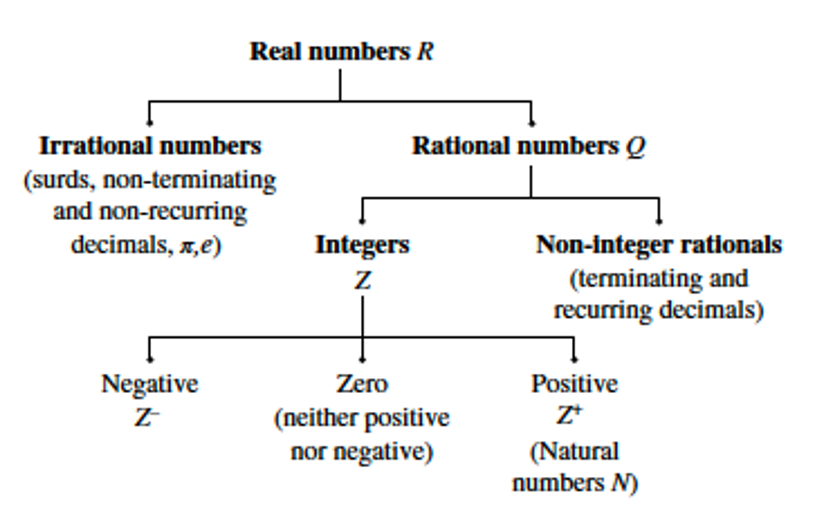
\includegraphics[scale=0.5]{number tree}
\end{center}

\section{Propositions}
A proposition or mathematical statement is a sentence that is either true or false.
\begin{center}
	\begin{tabular}{c|c|c}
		Symbol                & Meaning                   & Explanation                                                                \\ \hline
		$P \implies Q$        & Implication               & $P$ implies $Q$                                                            \\
		$\lnot A$             & Negation                  & The opposite of $A$                                                        \\
		$\forall x$           & Universal quantifier      & For all values of $x$                                                      \\
		$\exists $            & Existential quantifier    & There exists for some values of $x$                                        \\
		$P \Leftrightarrow Q$ & Equivalence               & The converse implication of $P \implies Q$ and $Q \implies P$ is also true \\
		$A \cap B$            & Union                     & $A$ or $B$                                                                 \\
		$A \cup B$            & Inter1                    & $A$ and $B$                                                                \\
		$A > B$               & Greater than              & $A$ is larger than $B$                                                     \\
		$A < B$               & Less than                 & $A$ is smaller than $B$                                                    \\
		$A \leq B$            & Less than and Equal to    & $A$ is smaller than or equal to $B$                                        \\
		$A \geq B$            & Greater than and Equal to & $A$ is larger than or equal to $B$                                         \\
		$A = B$               & Equal to                  & $A$ is the same value as $B$                                               \\
		$A \in \mathbb{N}$    & Contained in              & $A$ is contained in the set of natural numbers                             \\
	\end{tabular}
\end{center}

\section{Rules of equality}
Equality must follow these rules
\begin{center}
	Transitive property:
	\[
		\begin{array}{r@{}l}
			a + b \\
			b + c
		\end{array}
		\rbrace \implies a = c
	\]
	Substitution:
	\[
		\begin{array}{r@{}l}
			a + b = c \\
			b = d
		\end{array}
		\rbrace \implies a + d = c
	\]
	Matching:
	\[
		\begin{array}{r@{}l}
			a + b  = c \\
			a + d = c
		\end{array}
		\rbrace \implies b = d
	\]
	Adding equals:
	\[
		\begin{array}{r@{}l}
			a = b \\
			c=d
		\end{array}
		\rbrace \implies a + c = b + d
	\]
\end{center}

\section{Proof by contraposition}
Proof by contraposition is done by proving the contrapositive.  The contrapositive of a proposition is:
If $Q$, than $P$ becomes: If not $Q$, then not $P$

\section{Proof by contradiction}
Proof by contradiction is done by assuming that it is false initially.
\begin{enumerate}
	\item Assume (incorrectly) that what we want to prove is true, is actually false
	\item Show that the assumption eventually leads to mathematical nonsense
	\item Conclude that we are wrong to assume it is false
	\item realize that if it is not false, then it must be true
\end{enumerate}
Example:\\
$x$ satisfies $5^x = 2$, show that $x$ is irrational.
\begin{enumerate}
	\item Assume that $x$ is rational.
	\item $x = \frac{p}{q}, \in \mathbb{Z} (\text{with no common factors})$ as all rational numbers can be represented by a fraction of integers
	\item $5^{\frac{p}{q}} = 2$
	\item $(5^{\frac{p}{q}})^q = (2)^q$
	\item $5^p = 2^p$
	\item odd = even
	\item $\therefore$ Contradiction, assumption was wrong.
	\item $\therefore$ $x$ is irrational.
\end{enumerate}

\chapter{Circles}
\section{Terms}
Some important terms used with circles are:
\begin{center}
	\begin{tabular}{c|c}
		Term                 & Meaning                                                                                 \\ \hline
		Circumference        & The distance around the circle, or it's perimeter                                       \\
		Centre               & The point denoted $O$ which is the middle point of the circle                           \\
		Chord                & A line between two points on the circumference                                          \\
		Diameter             & The length of a chord that intersects the centre                                        \\
		Radius               & The length from the centre to the circumference                                         \\
		Arc                  & The part of a circle created by a chord $\arc{abd}$ is 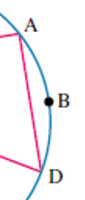
\includegraphics[scale=0.3]{arc} \\
		Angle at the centre  & The angle made by two radii                                                             \\
		Secant               & A line the cuts the circumference of the circle at two points                           \\
		Tangent              & A line that touches the circle at a point                                               \\
		Segment              & A region of a circle cut by a chord                                                     \\
		Cyclic quadrilateral & A quadrilateral (shape with four sides) whose vertices all lie on a circle              \\
	\end{tabular}
\end{center}

\section{Theorems}
\begin{center}
	\begin{tabular}[center]{|p{5cm}|p{3cm}|p{2cm}|}
		\hline
		Theorem                                                                                                              & Diagram                                       & Symbol                                               \\ \hline
		The angle at the centre of the circle is twice the angle at the circumference subtended on the same arc.             & 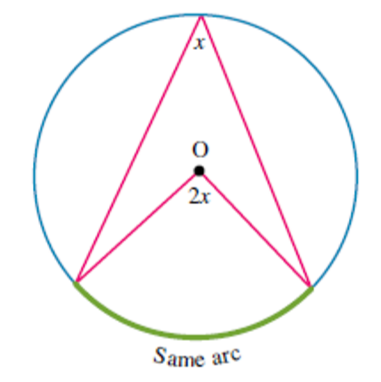
\includegraphics[width=3cm]{circle theorem 1} & 
\includegraphics[width=2cm]{circle theorem 1 symbol} \\ \hline
		Angles at the circumference subtended by the same arc are congruent.                                                 & 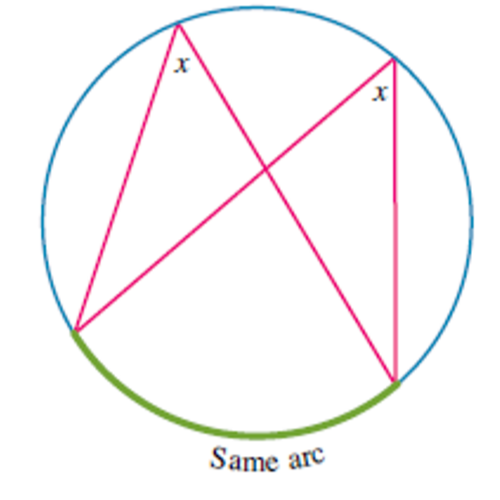
\includegraphics[width=3cm]{circle theorem 2} & 
\includegraphics[width=2cm]{circle theorem 2 symbol} \\ \hline
		The angle in a semicircle is a right angle.                                                                          & 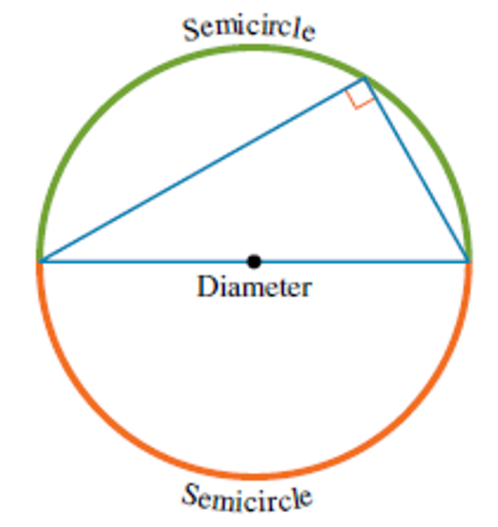
\includegraphics[width=3cm]{circle theorem 3} & 
\includegraphics[width=2cm]{circle theorem 3 symbol} \\ \hline
		If a line from the center bisects a chord, it is perpendicular to the chord.  The converse implication is also true. & 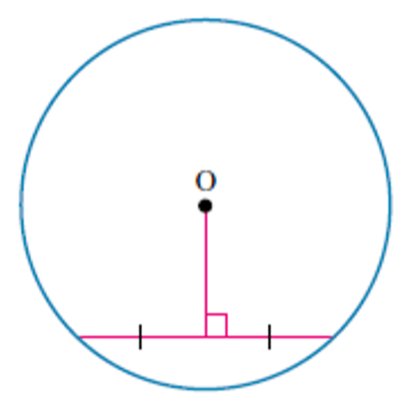
\includegraphics[width=3cm]{circle theorem 4} & 
\includegraphics[width=2cm]{circle theorem 4 symbol} \\ \hline
		If the chords are congruent, then they are equidistant from the centre of the center.                                & 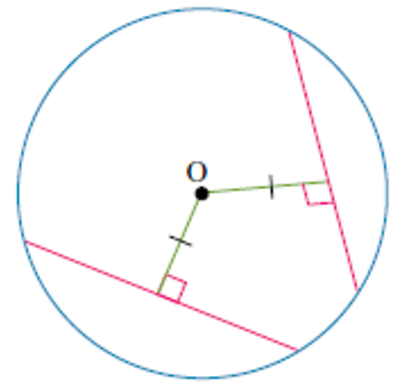
\includegraphics[width=3cm]{circle theorem 5} & 
\includegraphics[width=2cm]{circle theorem 5 symbol} \\ \hline
	\end{tabular}
	\begin{tabular}[center]{|p{5cm}|p{3cm}|p{2cm}|}
		\hline
		Theorem                                                                                                                                                                                  & Diagram                                        & Symbol                                                \\ \hline
		If two chords intersect inside the circle, then the point of inter1 divides each chord into two segments so that the product of the lengths of the segments for both chords is the same. & 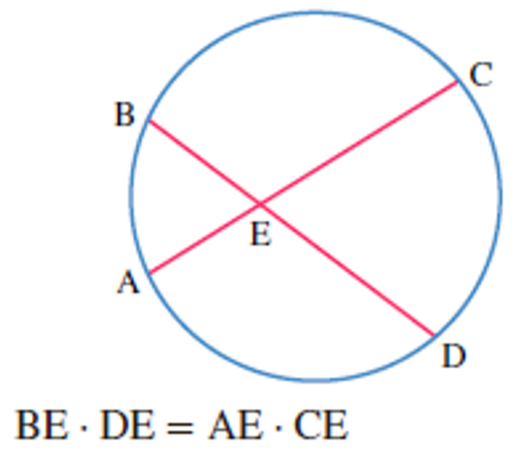
\includegraphics[width=3cm]{circle theorem 6}  & 
\includegraphics[width=2cm]{circle theorem 6 symbol}  \\ \hline
		If chords are congruent, they subtend equal angles at the centre.                                                                                                                        & 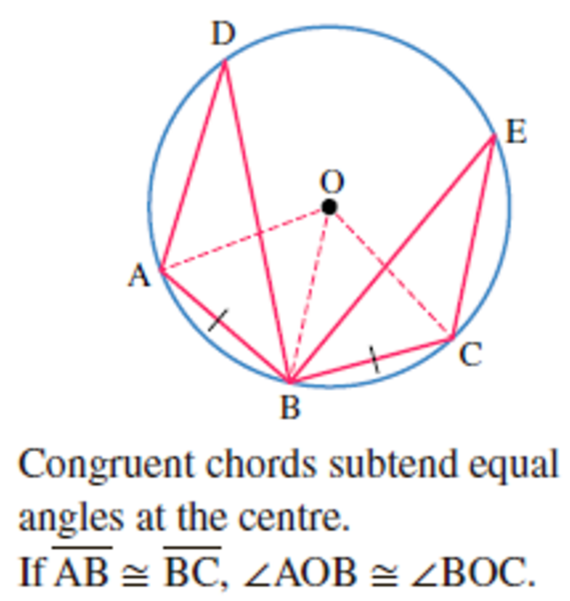
\includegraphics[width=3cm]{circle theorem 7}  & 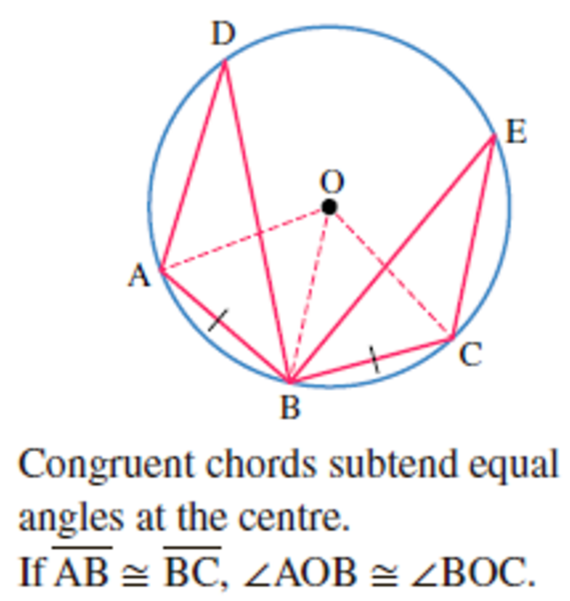
\includegraphics[width=2cm]{circle theorem 7 symbol}  \\ \hline
		A tangent and a radius intersects at right angles.                                                                                                                                       & 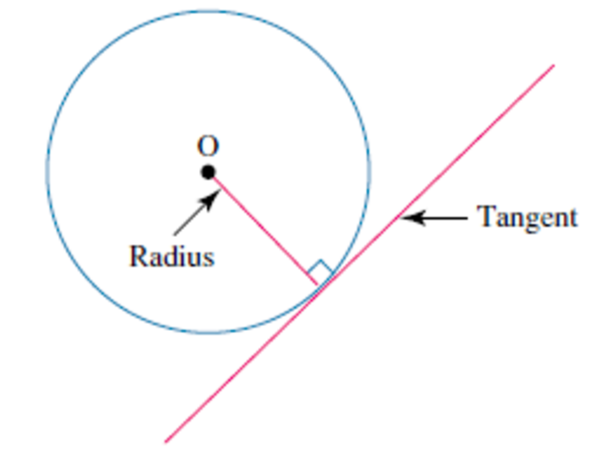
\includegraphics[width=3cm]{circle theorem 8}  & 
\includegraphics[width=2cm]{circle theorem 8 symbol}  \\ \hline
		Two tangents drawn from an external point to a circle are congruent.                                                                                                                     & 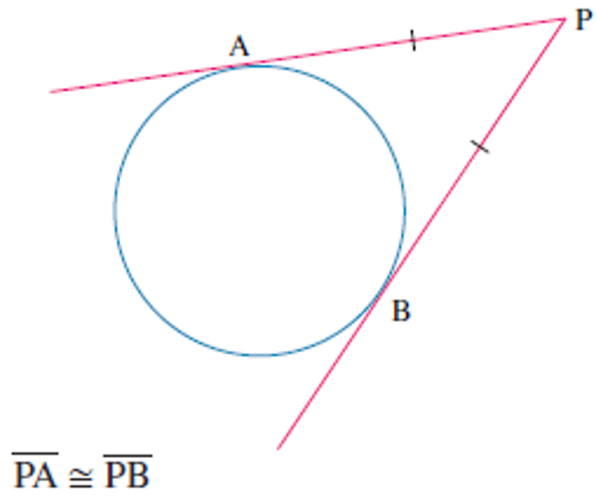
\includegraphics[width=3cm]{circle theorem 9}  & 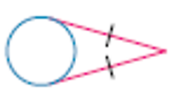
\includegraphics[width=2cm]{circle theorem 9 symbol}  \\ \hline
		The angle formed by two tangents meeting at an external point is bisected by a straight line joining the centre of the circle to that external point.                                    & 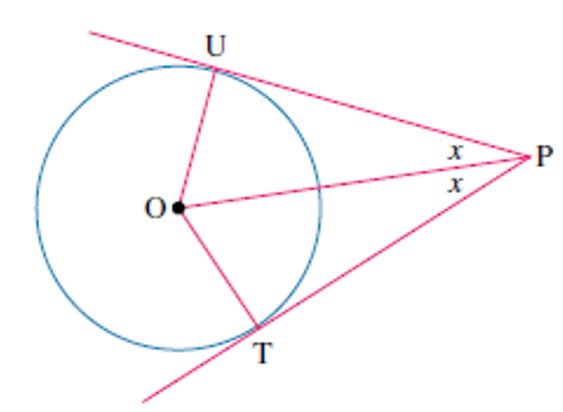
\includegraphics[width=3cm]{circle theorem 10} & 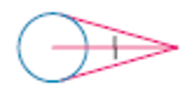
\includegraphics[width=2cm]{circle theorem 10 symbol} \\ \hline
	\end{tabular}
	\begin{tabular}[center]{|p{5cm}|p{3cm}|p{2cm}|}
		\hline
		Theorem                                                                                                                                                                                                                      & Diagram                                        & Symbol                                                \\ \hline
		The angle formed by a tangent and a chord is congruent to the angle in the alternate segment.                                                                                                                                & 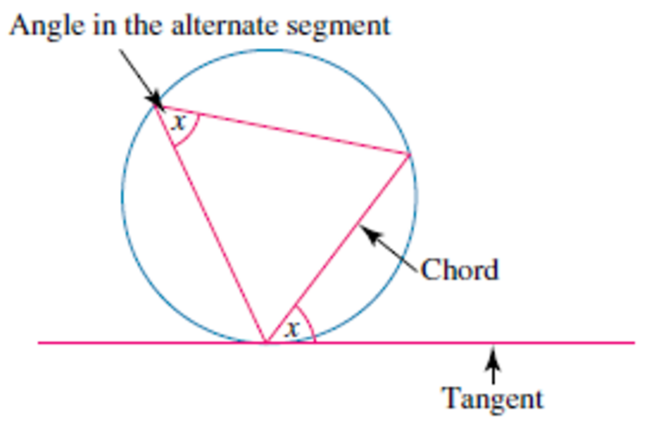
\includegraphics[width=3cm]{circle theorem 11} & 
\includegraphics[width=2cm]{circle theorem 11 symbol} \\ \hline
		If a secant (meeting the circle at A and B) and a tangent (meeting at circle at T) are drawn from an external point P, the square of the length of the tangent equals the product of the length to the circle on the secant. & \includegraphics[width=3cm]{circle theorem 12} & \includegraphics[width=2cm]{circle theorem 12 symbol} \\ \hline
		If two secants intersect outside the circle, then the product of one external secant segment length and it's external length is equal to the product of the other secant lengths.                                            & \includegraphics[width=3cm]{circle theorem 13} & \includegraphics[width=2cm]{circle theorem 13 symbol} \\ \hline
		The opposite angles of a cyclic quadrilateral are supplementary.                                                                                                                                                             & \includegraphics[width=3cm]{circle theorem 14} & \includegraphics[width=2cm]{circle theorem 14 symbol} \\ \hline
		The exterior angle of a cyclic quadrilateral is congruent to the inner opposite angle.                                                                                                                                       & \includegraphics[width=3cm]{circle theorem 15} & \includegraphics[width=2cm]{circle theorem 15 symbol} \\ \hline
	\end{tabular}
\end{center}

\chapter{Complex numbers}
\section{The imaginary numbers}
The unit for the imaginary numbers is donated the letter $i$.  $i$ is equal to $\sqrt[2]{-1}$\\

As in, $i^2 = -1$.  As the powers of $i$ increases, it rotates $\frac{1}{2}\pi$ through the Argand plane:
\begin{align*}
	i^0 & = 1  \\
	i^1 & = i  \\
	i^2 & = -1 \\
	i^3 & = -i \\
	i^4 & = 1  \\
	i^5 & = i  \\
	i^6 & = -1 \\
	i^7 & = -i
\end{align*}
\begin{center}
	\begin{tikzpicture}[scale=1.2]
		\begin{axis}[
				axis lines=middle,
				xmin=-3, xmax=3,
				ymin=-3, ymax=3,
				xtick={-1,0,1},
				ytick={-1,0,1},
				xlabel={$\Re$},
				ylabel={$\Im$},
			]
			\addplot [thick,->, red] coordinates {(0,0) (1,0)} node[below right] {$1$};
			\addplot [thick,->, red!75!purple] coordinates {(0,0) (0,1)} node[above left] {$i$};
			\addplot [thick,->, red!50!purple] coordinates {(0,0) (-1,0)} node[below left] {$-1$};
			\addplot [thick,->, red!25!purple] coordinates {(0,0) (0,-1)} node[below right] {$-i$};
			\addplot [thick,->, purple] coordinates {(0,0) (2,0)} node[below right] {$2$};
			\addplot [thick,->, purple!75!red] coordinates {(0,0) (0,2)} node[above left] {$2i$};
			\addplot [thick,->, purple!50!red] coordinates {(0,0) (-2,0)} node[below left] {$-2$};
			\addplot [thick,->, purple!25!red] coordinates {(0,0) (0,-2)} node[below right] {$-2i$};
			\node at (axis cs:1.5,.5) {$\times i^0$};
			\node at (axis cs:.5,1.5) {$\times i^1$};
			\node at (axis cs:-1.5,.5) {$\times i^2$};
			\node at (axis cs:.5,-1.5) {$\times i^3$};
			\draw [thick,-stealth,bend right=90,color=red] (axis cs: 1.05,-.05) to (axis cs: .05,.95);
			\draw [thick,-stealth,bend right=90,color=red!75!purple] (axis cs: .05,.95) to (axis cs: -1.05,.05);
			\draw [thick,-stealth,bend right=90,color=red!50!purple] (axis cs: -1.05,.05) to (axis cs: -.05,-.95);
			\draw [thick,-stealth,bend right=90,color=red!25!purple] (axis cs: -.05,-.95) to (axis cs: 1.05,-.05);
			\node at (axis cs:.5,.5) {$\times i$};
			\node at (axis cs:-.5,.5) {$\times i$};
			\node at (axis cs:-.5,-.5) {$\times i$};
			\node at (axis cs:.5,-.5) {$\times i$};
		\end{axis}
	\end{tikzpicture}
\end{center}

\section{Complex numbers}
Compleax numbers usually denoted the letter $Z$, and are numbers which lie on the Argand plane.  They have an imaginary component and a real component:
\[
	Z := a + b \times i, (a, b \in \Re)
\]

\section{Basic operations}
\subsection{Addition}
To add a complex number, add the real and imaginary part seperately:
\[
	\text{let: } Z := 3 + 2i, C := 8 + 7i
\]
\begin{align*}
	Z + C & = (Re(Z) + Re(C)) + (Im(Z) + Im(C))i \\
	      & = (3 + 8) + (2 + 7)i                 \\
	      & = 11 + 9i
\end{align*}

\subsection{Subtraction}
To subtract a complex number, use the same formula as the addition:
\[
	\text{let: } Z := 3 + 2i, C := 8 + 7i
\]
\begin{align*}
	Z - C & = (Re(Z) + Im(Z)i) + -(Re(C) + Im(C)i) \\
	      & = Re(Z) + Im(Z)i - Re(C) - Im(C)i      \\
	      & = Re(Z) - Re(C) + (Im(Z) - Im(C))i     \\
	      & = 3 - 8 + (2 - 7)i                     \\
	      & = -5 - 5i
\end{align*}

\subsection{Multiplication by a scaler}
\[
	\text{let: } k := 3, Z = 3 + 2i
\]
\begin{align*}
	k \times Z & = k(3 + 2i) \\
	           & = 3(3 + 2i) \\
	           & = 9 + 6i
\end{align*}

\subsection{Multiplication by another complex number}
Let: $z := a + bi, w := c + di$
\begin{align*}
	zw & = (a \times c - b \times d) + (a \times d + b \times c)i \\
	zw & = (6 - c0) + (1d + 8)i                                   \\
	zw & = -1b + cai
\end{align*}

\section{Complex conjugates}
The conjugate is as follows:
\begin{center}
	Let: $z := a + bi$\\
	$\therefore$ the conjugate, or $\bar{z}$:\\
	$\bar{z} := a - bi$.
\end{center}

\section{Division of complex numbers}
Let: $z := a + bi, w := c + di$
\begin{align*}
	\frac{z}{w} & = \frac{a + bi}{c + di}\\
	& = \frac{a + bi}{c + di} \times \frac{\bar{w}}{\bar{w}}\\
	& = \frac{a + bi}{c + di} \times \frac{c - di}{c - di}\\
	& = \frac{ac + }{}
\end{align*}

\section{The multiplicative inverse}

\section{The Argand plane}
\subsection{The representation of complex numbers as a vector}

\section{Polar form}

\subsection{The argument}

\subsection{Multiplication}

\subsection{Division}

\subsection{Powers}

\subsection{Quadratic equations}

\chapter{Functions}
\section{Absolute value functions}

\section{Modulus functions}

\section{Reciprocal functions}

\section{Rational functions}

\chapter{Trigonometric identities}
\section{Angles}

\section{General solutions to the basic ratios}

\section{Reciprocal functions}

\section{Pythagorian identities}

\section{Compound/angle sum and angle difference formulas}

\section{Double angle formulas}

\section{Half angle formulas}

\section{Sum-angle identities}

\section{Sum of two trigonometric ratios}

\section{Multiple angle formulas}
\subsection{De Moivre's theorem}

\chapter{Matricies}
\section{Addition and subtraction}

\section{Scalar multiplication}

\section{Matrix multiplication}

\section{Determanents}

\section{Inverse matricies}

\section{Simuletanious equations}

\section{Transformations}
\subsection{Translations}

\subsection{Reflections}
\subsubsection{x-axis}

\subsubsection{y-axis}

\subsubsection{Line: $y = x$}

\subsubsection{Line: $y = -x$}

\subsubsection{Line: $y = x \tan(\theta)$}

\subsection{Rotations}
\subsubsection{Clockwise}

\subsubsection{Anti-Clockwise}

\subsection{Dialations}
\subsubsection{X-axis}

\subsubsection{Y-axis}

\section{Combined translations}



\chapter{Summation notation}



\chapter{Proofs}
\section{Proof by induction}
\begin{generalInformation}
    Proof by induction means that if one is true, they all must be true 
\end{generalInformation}
\begin{example}
    Let:
    \[
        1 + 2 + 3 + ... + n = \frac{n(n + 1)}{2}, n \greq 1
    \]
    
\end{example}

\section{Proof by divisibility}


\end{document}
